%! Author = tobias
%! Date = 18.06.22

% Preamble
\documentclass[11pt]{article}

% Packages
\usepackage{amsmath}
\usepackage{amsfonts}
\usepackage{graphicx}
\title{Statistical Learning Methods \\ Questions Lecture 3}
\author{Tobias Famos}
% Document
\begin{document}
    \maketitle
    \subsection*{Questions}
    \begin{enumerate}
        \item What is a Linear Simple Regression Model?
        \item When do you use a simple linear regression?
        \item How do you determine, which linear function to use?
        \item Given the RSS, how do we compute the MSE?
        \item State model with two attributes, ($x_1$ and $x_2$)
        \item Interprete the following output and give the model to it. \\
        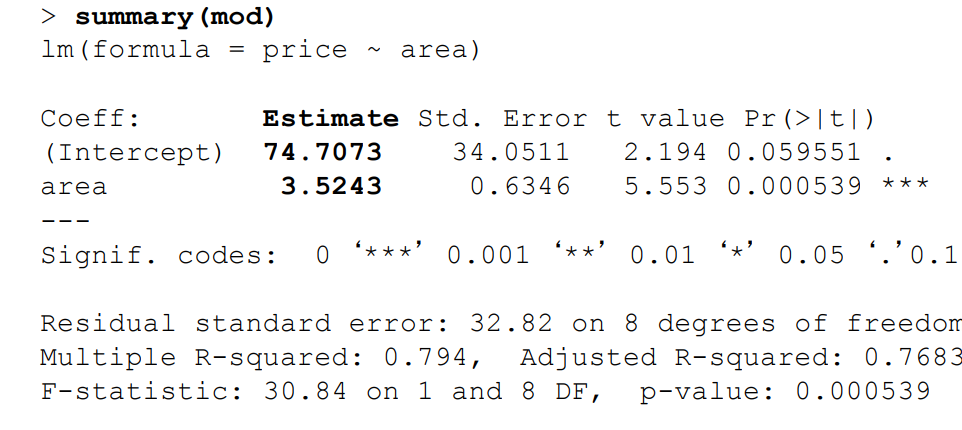
\includegraphics[scale=0.3]{pictures/linreg1}
        \item Give the confidence intervall for the area (above)
        \item Explain $\text{R}^2$
    \end{enumerate}
    \newpage
    \subsection*{Answers}
    \begin{enumerate}
        \item The linear simple regression model approximates data with a linear function $f(x)$.
        \item \begin{itemize}
                  \item Either when the dependence of $Y$ to $X$ is linear.
                  \item Or as the first approximation of data as the model is quite easy and quick.
        \end{itemize}
        \item \begin{itemize}
                  \item The \textbf{least squares method} can be used to test different functions and get a numeric error.
                  \item We choose the function in a way, that it minimizes the RSS (Residual Sum of Squares).
        \end{itemize}
        \item The Media Standard Error (MSE) can be computed form the Residual Sum of Squares (RSS) by dividing by $n$
        \item $y = \beta_0 + \beta_1 \cdot x_1 + \beta_2 \cdot x_2 + \epsilon$
        \item \begin{itemize}
                  \item Model: $\text{price} = 74.7 + 3.52 \cdot \text{area}$
                  \item The Model is significant (p-value: 0.05 \%) is smaller than 5\%
                  \item 8 degrees of Freedom means there were 9 data points
                  \item The area is highly significant, the intercept is almost significant
        \end{itemize}
        \item \begin{itemize}
                  \item Defined by $\hat{\beta}_i \pm 2 \cdot \hat{\sigma}_{\beta_i}$
                  \item Thus: $3.52 \pm 2 \cdot 0.63$ = $[2.26, 4.78]$
        \end{itemize}
        \item     \begin{itemize}
                      \item It states how much of the variance is explained in the model.
                      \item Formula: $R^2 = 1 - \frac{RSS}{TSS}$ Where TSS = Total sum of squares, meaning the variance
                      of the sample.
        \end{itemize}
    \end{enumerate}
\end{document}